\begin{lstLNat}
    fonction existeArc(i : entier, j : entier, G : graphe) : booléen
    debut
        retourner appartient(j, G.listeArcsSortants[i])
    fin
\end{lstLNat}

\includegraphics[width=0.5\textwidth]{figures/ex7-1.jpg}

\begin{lstLNat}
    fonction ajoutArc(i : entier, j : entier, G : graphe)
    debut
        si non(existeArc(i, j, G)) faire
        debut
            G.listeArcsSortants = ajouter(j, listeArcsSortants)
        fin
    fin
\end{lstLNat}
    
\includegraphics[width=0.5\textwidth]{figures/ex7-2.jpg}

\begin{lstLNat}
    fonction supprimerArc(i : entier, j : entier, G : graphe)
    debut
        si existeArc(i, j, G) faire
        debut
            G.listeArcsSortants = ajouter(j, G.listeArcsSortants)
        fin
    fin
\end{lstLNat}

% ================= APRES =================
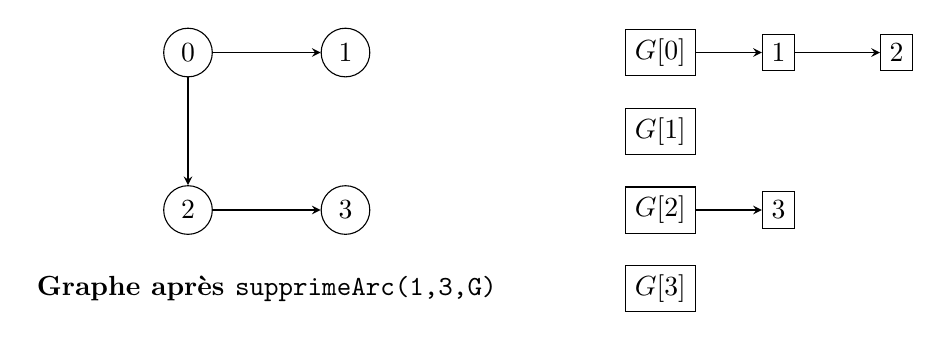
\begin{tikzpicture}[>=stealth]

% --- Graphe ---
\node[circle, draw] (n0) at (0,0) {0};
\node[circle, draw] (n1) at (2,0) {1};
\node[circle, draw] (n2) at (0,-2) {2};
\node[circle, draw] (n3) at (2,-2) {3};

\draw[->] (n0) -- (n1);
\draw[->] (n0) -- (n2);
\draw[->] (n2) -- (n3);

\node at (1,-3) {\textbf{Graphe après \texttt{supprimeArc(1,3,G)}}};

% --- Tableau de listes ---
\node[draw, rectangle] (g0) at (6,0) {$G[0]$};
\node[draw, rectangle] (g01) at (7.5,0) {1};
\node[draw, rectangle] (g02) at (9,0) {2};

\node[draw, rectangle] (g1) at (6,-1) {$G[1]$};

\node[draw, rectangle] (g2) at (6,-2) {$G[2]$};
\node[draw, rectangle] (g23) at (7.5,-2) {3};

\node[draw, rectangle] (g3) at (6,-3) {$G[3]$};

\draw[->] (g0) -- (g01);
\draw[->] (g01) -- (g02);
\draw[->] (g2) -- (g23);

\end{tikzpicture}